\section{Results}
\label{sec:results}

After successfully pre-processing the Pima Indians Diabetes dataset and training our model, we evaluated its performance to assess its generalization and effectiveness in diabetes prediction.

\subsection*{Training Performance}

The dataset was split into 80\% training and 20\% testing partitions. We employed early stopping with a patience of 20 epochs to prevent overfitting. This halted training once the validation loss ceased to improve. The final model architecture included three hidden layers of 32, 16, and 8 neurons, interleaved with dropout layers to improve regularization.

The model was trained over 100 epochs with a batch size of 16 using the Adam optimizer and binary cross-entropy as the loss function. The best-performing model, based on validation loss, achieved a test (validation) accuracy of approximately \textbf{81\%}.

\subsection*{Evaluation Metrics}
In addition to accuracy, we computed precision, recall, and F1-score to provide a more comprehensive assessment, particularly due to the dataset’s mild class imbalance. These metrics are summarized in Table~\ref{tab:metrics}.

\begin{table}[h]
\centering
\caption{Evaluation Metrics on Test Set}
\label{tab:metrics}
\begin{tabular}{|c|c|}
\hline
\textbf{Metric} & \textbf{Score} \\
\hline
Accuracy & 83\% \\
Precision (Non-Diabetic) & 83\% \\
Recall (Non-Diabetic) & 80\% \\
F1-Score (Non-Diabetic) & 81\% \\
\hline
Precision (Diabetic) & 77\% \\
Recall (Diabetic) & 72\% \\
F1-Score (Diabetic) & 74\% \\
\hline
\end{tabular}
\end{table}

\subsection*{Visualization of Results}
To understand the behavior across multiple of our original (non-optimal) models, matplotlib was used to generate graphs showing the training precision and the validation precision, as seen in Figures 1, 2, and 3 below. These graphs show the dramatic change across models.

\begin{figure}[h]
    \centering
    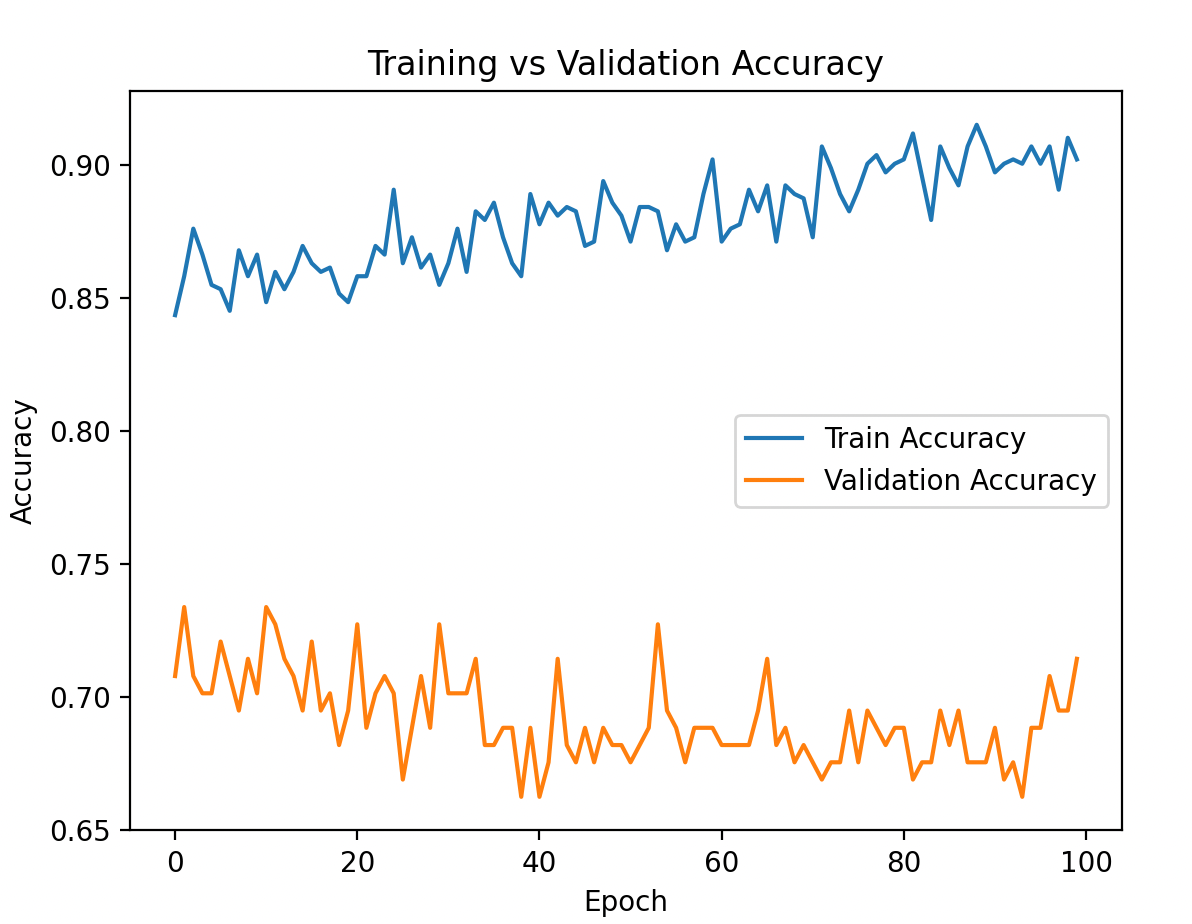
\includegraphics[width=0.4\textwidth]{project-report/chapters/figures/model 1.png}
    \caption{Testing vs Validation Accuracy: Model 1}
\end{figure}

\begin{figure}[h]
    \centering
    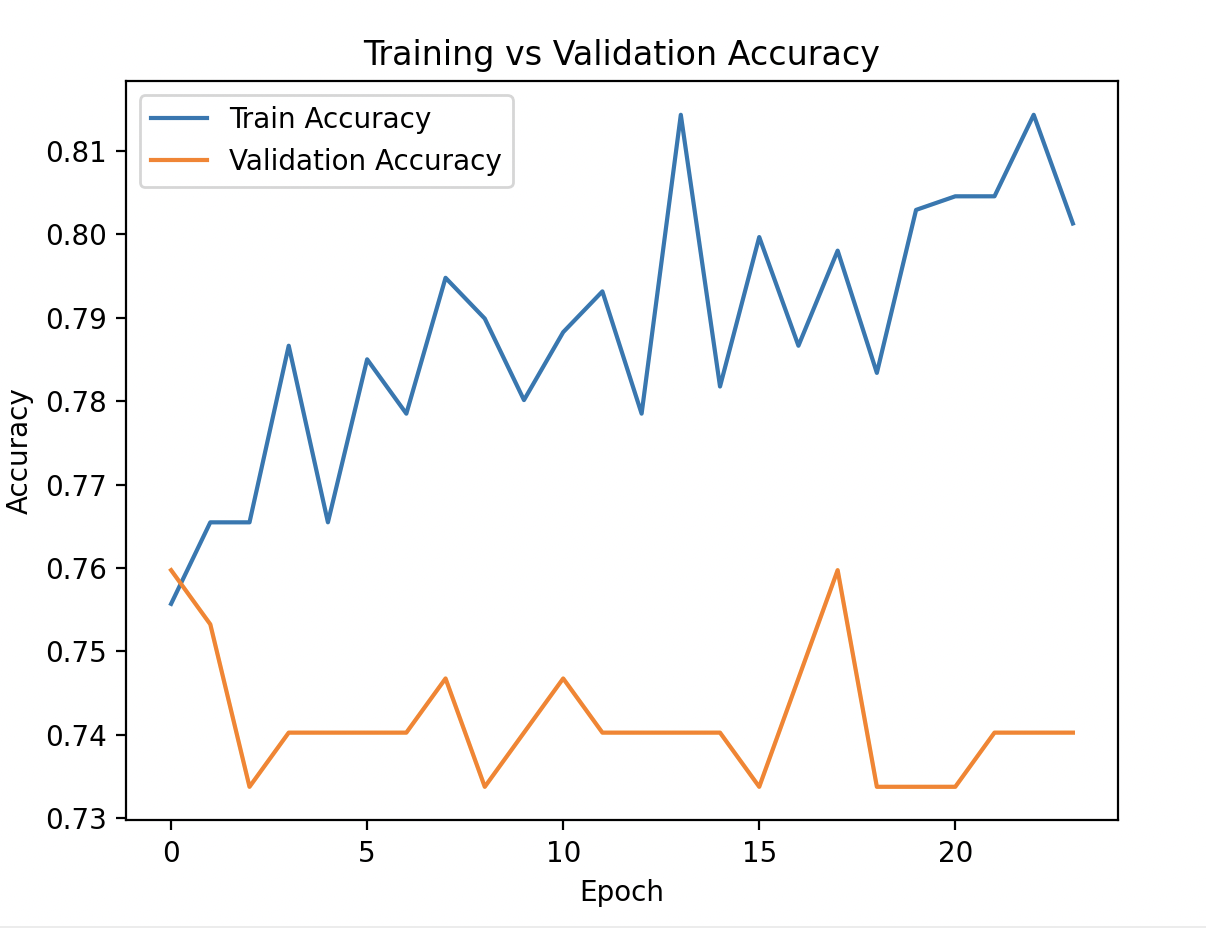
\includegraphics[width=0.4\textwidth]{project-report/chapters/figures/model 2.png}
    \caption{Testing vs Validation Accuracy: Model 2}
\end{figure}

\begin{figure}[h]
    \centering
    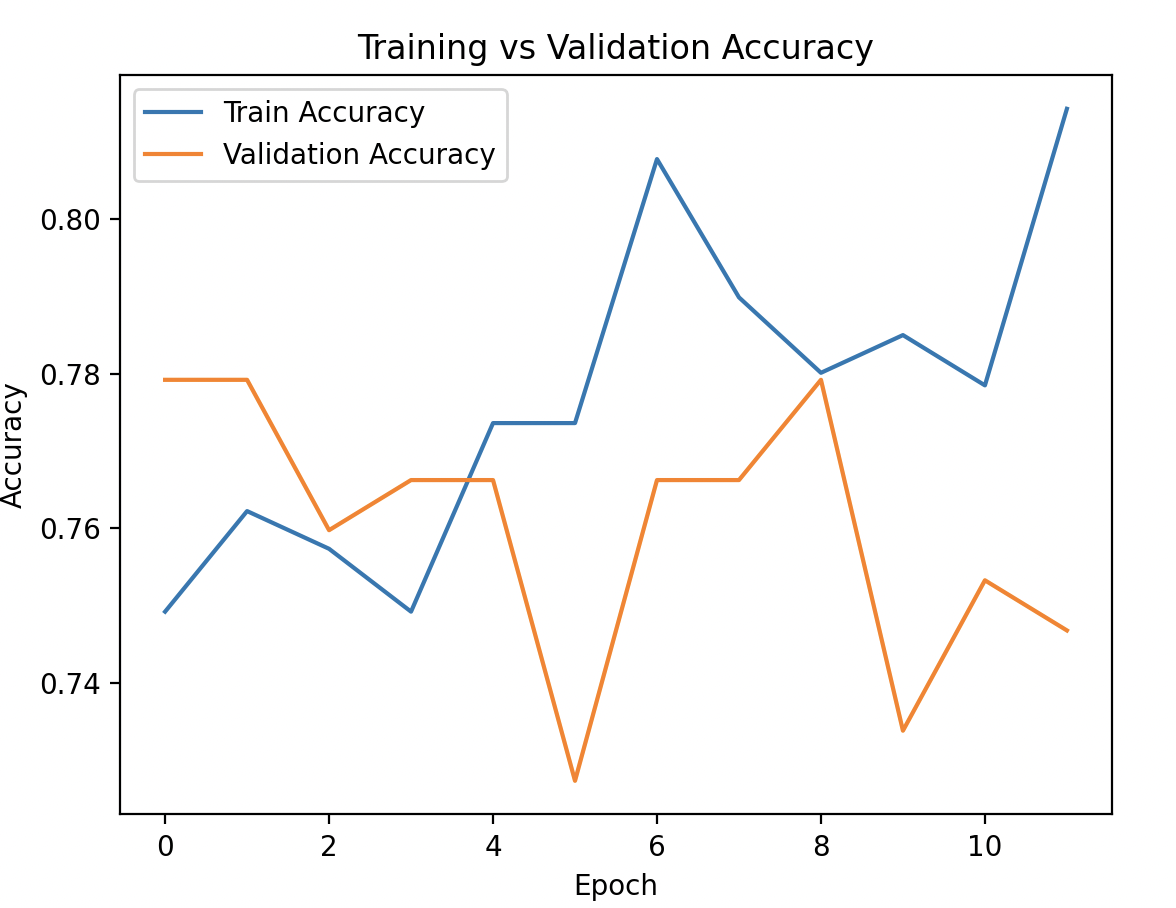
\includegraphics[width=0.4\textwidth]{project-report/chapters/figures/model 3.png}
    \caption{Testing vs Validation Accuracy: Model 3}
\end{figure}
